\section{Classer des angles (4 points)}

\begin{questions}
	\question[4] Pour chaque angle ci-dessous, remplir \textbf{sur cette feuille  }le tableau suivant avec ses différentes caractéristiques.
	
	 \begin{center}
	 	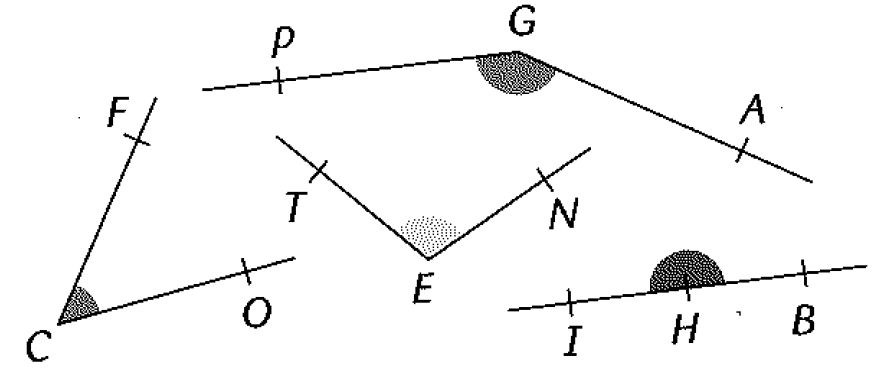
\includegraphics[scale=0.4]{img/angles}
	 \end{center}

\begin{tabular}{|c|c|c|c|}
	\hline
	\textbf{Angle} & \textbf{Sommet} & \textbf{Côtés} & \textbf{Type} \\ \hline
	&                 &                &               \\ \hline
	&                 &                &               \\ \hline
	&                 &                &               \\ \hline
	&                 &                &               \\ \hline
	%&                 &                &               \\ \hline
\end{tabular}

\end{questions}